\documentclass{standalone}
\usepackage{tikz}
\usetikzlibrary{patterns, positioning}
\usepackage[sfdefault]{ClearSans} %% option 'sfdefault' activates Clear Sans as the default text font
\usepackage[T1]{fontenc}

\begin{document}
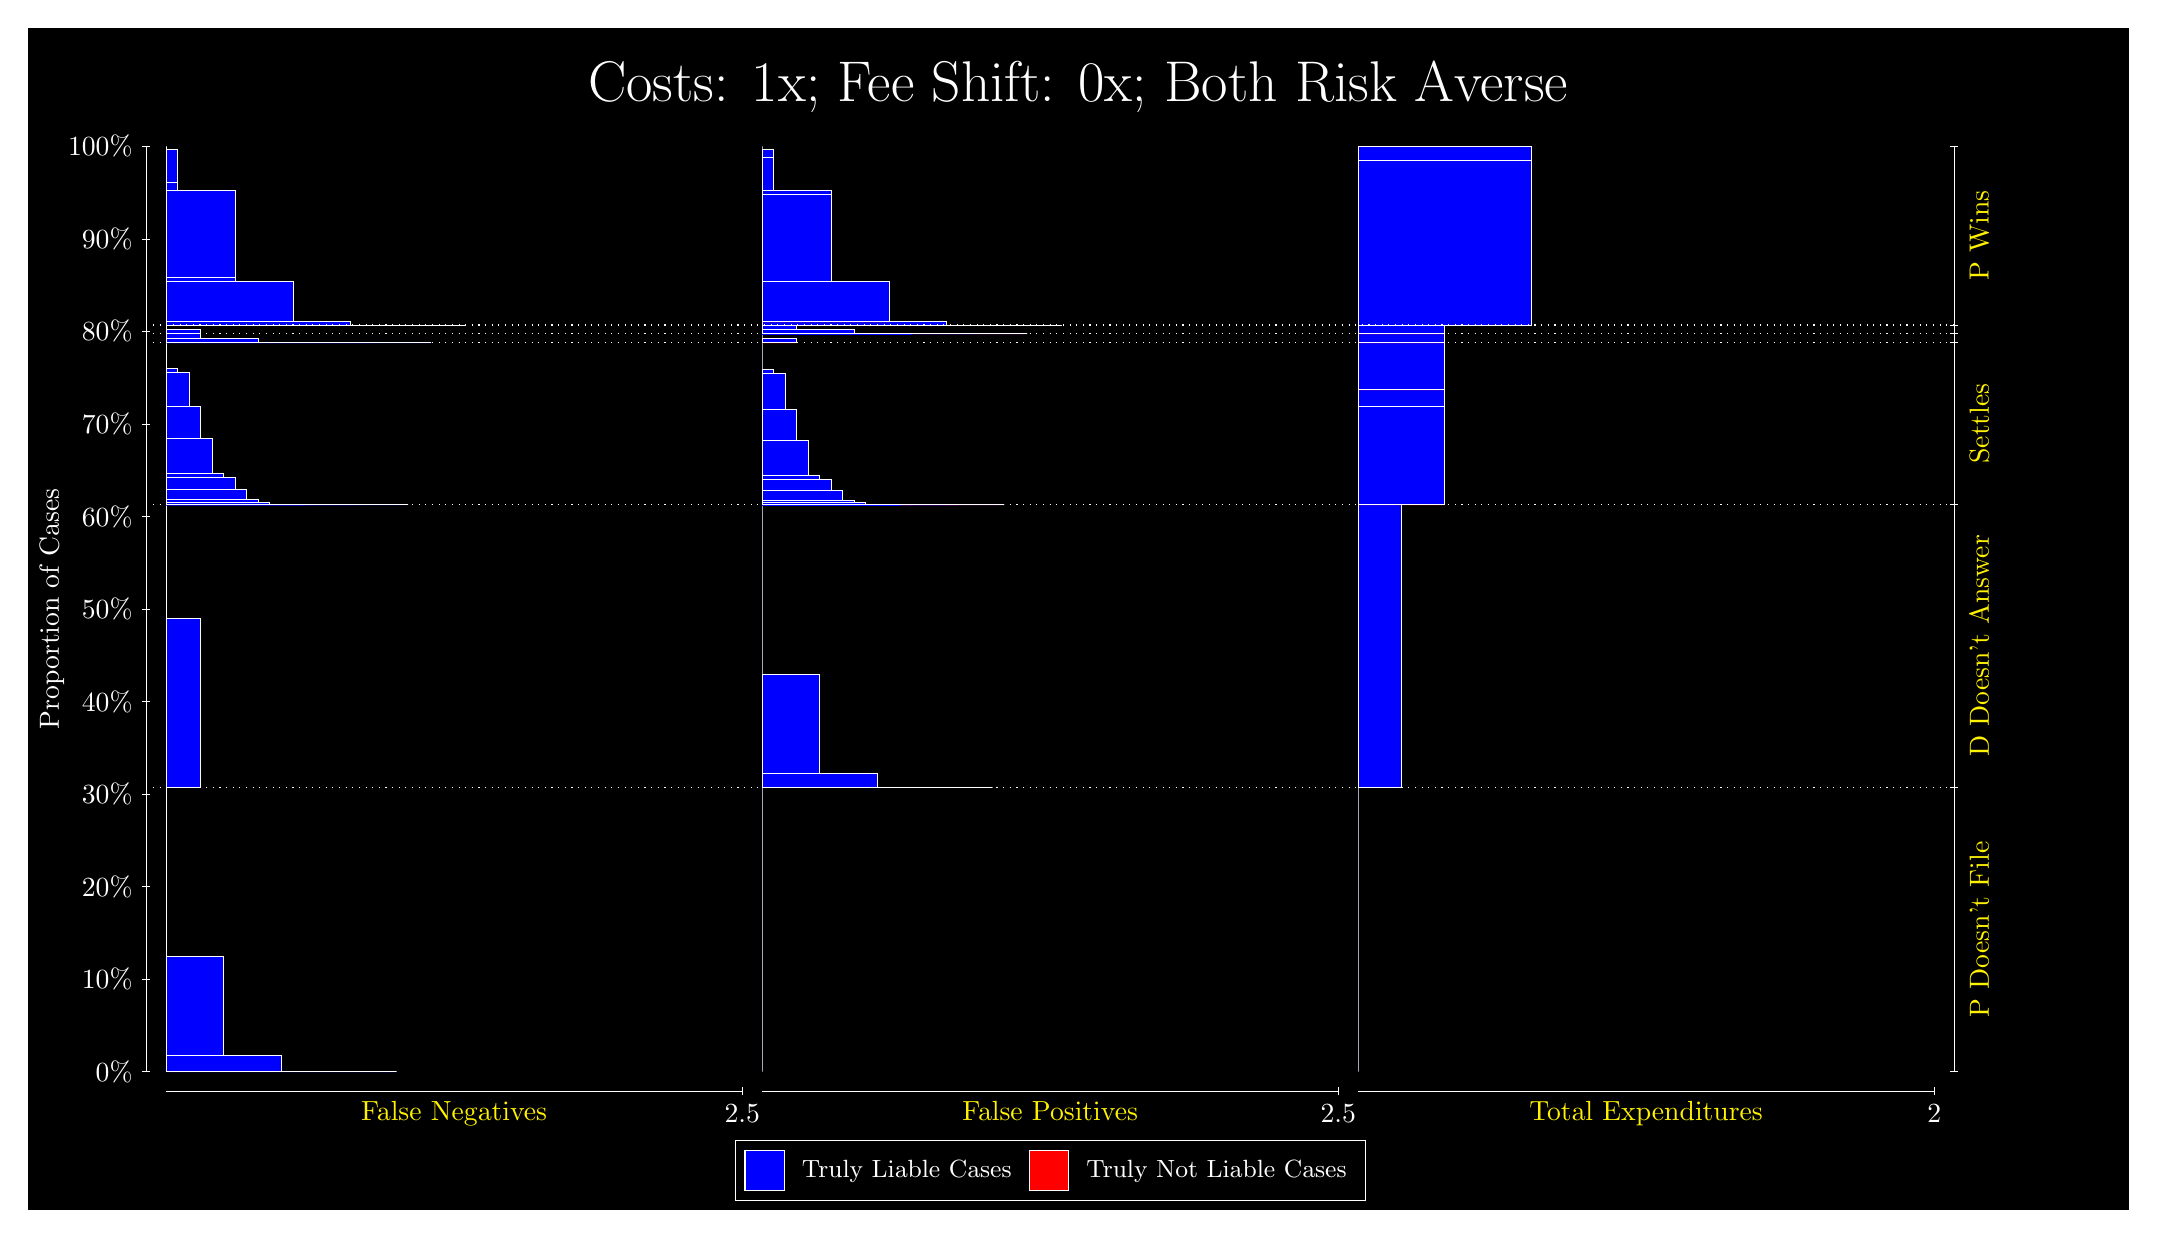
\begin{tikzpicture}
\draw[fill=black] (0,0) rectangle (26.667,15);
\draw[text=white] (0,13.5) rectangle (26.667,15) node[midway] {\huge Costs: 1x; Fee Shift: 0x; Both Risk Averse};
\draw[white, very thin] (1.5,1.75) -- (1.5,13.5);
\node[rotate=90, text=white, anchor=center] at (0.3, 7.625) {Proportion of Cases};
\draw[white, very thin] (1.45,1.75) -- (1.55,1.75);
\node[text=white, anchor=east] at (1.45, 1.75) {0\%};
\draw[white, very thin] (1.45,2.925) -- (1.55,2.925);
\node[text=white, anchor=east] at (1.45, 2.925) {10\%};
\draw[white, very thin] (1.45,4.1) -- (1.55,4.1);
\node[text=white, anchor=east] at (1.45, 4.1) {20\%};
\draw[white, very thin] (1.45,5.275) -- (1.55,5.275);
\node[text=white, anchor=east] at (1.45, 5.275) {30\%};
\draw[white, very thin] (1.45,6.45) -- (1.55,6.45);
\node[text=white, anchor=east] at (1.45, 6.45) {40\%};
\draw[white, very thin] (1.45,7.625) -- (1.55,7.625);
\node[text=white, anchor=east] at (1.45, 7.625) {50\%};
\draw[white, very thin] (1.45,8.8) -- (1.55,8.8);
\node[text=white, anchor=east] at (1.45, 8.8) {60\%};
\draw[white, very thin] (1.45,9.975) -- (1.55,9.975);
\node[text=white, anchor=east] at (1.45, 9.975) {70\%};
\draw[white, very thin] (1.45,11.15) -- (1.55,11.15);
\node[text=white, anchor=east] at (1.45, 11.15) {80\%};
\draw[white, very thin] (1.45,12.325) -- (1.55,12.325);
\node[text=white, anchor=east] at (1.45, 12.325) {90\%};
\draw[white, very thin] (1.45,13.5) -- (1.55,13.5);
\node[text=white, anchor=east] at (1.45, 13.5) {100\%};

\draw[white, very thin] (24.457,1.75) -- (24.457,13.5);
\draw[white, very thin] (24.407,1.75) -- (24.507,1.75);
\node[anchor=west] at (24.407, 1.75) {};
\draw[white, very thin] (24.407,5.3618) -- (24.507,5.3618);
\node[anchor=west] at (24.407, 5.3618) {};
\draw[white, very thin] (24.407,8.9491) -- (24.507,8.9491);
\node[anchor=west] at (24.407, 8.9491) {};
\draw[white, very thin] (24.407,11.008) -- (24.507,11.008);
\node[anchor=west] at (24.407, 11.008) {};
\draw[white, very thin] (24.407,11.12) -- (24.507,11.12);
\node[anchor=west] at (24.407, 11.12) {};
\draw[white, very thin] (24.407,11.231) -- (24.507,11.231);
\node[anchor=west] at (24.407, 11.231) {};
\draw[white, very thin] (24.407,13.5) -- (24.507,13.5);
\node[anchor=west] at (24.407, 13.5) {};

\draw[white, very thin, fill=blue] (1.75,1.75) rectangle (4.6775,1.75);
\draw[white, very thin, fill=blue] (1.75,1.75) rectangle (3.9457,1.7517);
\draw[white, very thin, fill=blue] (1.75,1.7517) rectangle (3.2138,1.9585);
\draw[white, very thin, fill=blue] (1.75,1.9585) rectangle (2.4819,3.213);
\draw[white, very thin, fill=red] (1.75,3.213) rectangle (1.75,3.213);
\draw[white, very thin, fill=blue] (1.75,3.213) rectangle (1.75,5.3618);
\draw[white, very thin, fill=blue] (1.75,5.3618) rectangle (2.1891,7.5116);
\draw[white, very thin, fill=red] (1.75,7.5116) rectangle (1.75,7.5116);
\draw[white, very thin, fill=blue] (1.75,7.5116) rectangle (1.75,8.9491);
\draw[white, very thin, fill=blue] (1.75,8.9491) rectangle (4.8239,8.9491);
\draw[white, very thin, fill=blue] (1.75,8.9491) rectangle (4.2384,8.9491);
\draw[white, very thin, fill=blue] (1.75,8.9491) rectangle (4.092,8.9491);
\draw[white, very thin, fill=blue] (1.75,8.9491) rectangle (3.6529,8.9492);
\draw[white, very thin, fill=blue] (1.75,8.9492) rectangle (3.5065,8.9494);
\draw[white, very thin, fill=blue] (1.75,8.9494) rectangle (3.3602,8.9559);
\draw[white, very thin, fill=blue] (1.75,8.9559) rectangle (3.0674,8.9814);
\draw[white, very thin, fill=blue] (1.75,8.9814) rectangle (2.921,9.0114);
\draw[white, very thin, fill=blue] (1.75,9.0114) rectangle (2.7746,9.1422);
\draw[white, very thin, fill=blue] (1.75,9.1422) rectangle (2.6283,9.2941);
\draw[white, very thin, fill=blue] (1.75,9.2941) rectangle (2.4819,9.3428);
\draw[white, very thin, fill=blue] (1.75,9.3428) rectangle (2.3355,9.7927);
\draw[white, very thin, fill=blue] (1.75,9.7927) rectangle (2.1891,10.193);
\draw[white, very thin, fill=blue] (1.75,10.193) rectangle (2.0428,10.634);
\draw[white, very thin, fill=blue] (1.75,10.634) rectangle (1.8964,10.684);
\draw[white, very thin, fill=red] (1.75,10.684) rectangle (1.75,10.684);
\draw[white, very thin, fill=blue] (1.75,10.684) rectangle (1.75,11.008);
\draw[white, very thin, fill=blue] (1.75,11.008) rectangle (5.1167,11.008);
\draw[white, very thin, fill=blue] (1.75,11.008) rectangle (4.3848,11.008);
\draw[white, very thin, fill=blue] (1.75,11.008) rectangle (3.6529,11.01);
\draw[white, very thin, fill=blue] (1.75,11.01) rectangle (2.921,11.066);
\draw[white, very thin, fill=blue] (1.75,11.066) rectangle (2.1891,11.12);
\draw[white, very thin, fill=red] (1.75,11.12) rectangle (1.75,11.12);
\draw[white, very thin, fill=blue] (1.75,11.12) rectangle (2.1891,11.174);
\draw[white, very thin, fill=red] (1.75,11.174) rectangle (1.75,11.174);
\draw[white, very thin, fill=blue] (1.75,11.174) rectangle (1.75,11.231);
\draw[white, very thin, fill=blue] (1.75,11.231) rectangle (5.5558,11.231);
\draw[white, very thin, fill=blue] (1.75,11.231) rectangle (4.8239,11.232);
\draw[white, very thin, fill=blue] (1.75,11.232) rectangle (4.092,11.272);
\draw[white, very thin, fill=blue] (1.75,11.272) rectangle (3.3602,11.787);
\draw[white, very thin, fill=blue] (1.75,11.787) rectangle (2.6283,11.835);
\draw[white, very thin, fill=blue] (1.75,11.835) rectangle (2.6283,12.944);
\draw[white, very thin, fill=blue] (1.75,12.944) rectangle (1.8964,13.042);
\draw[white, very thin, fill=blue] (1.75,13.042) rectangle (1.8964,13.459);
\draw[white, very thin, fill=red] (1.75,13.459) rectangle (1.75,13.459);
\draw[white, very thin, fill=blue] (1.75,13.459) rectangle (1.75,13.5);
\draw[white, very thin, fill=red] (9.3189,1.75) rectangle (9.3189,1.75);
\draw[white, very thin, fill=blue] (9.3189,1.75) rectangle (9.3189,5.3618);
\draw[white, very thin, fill=red] (9.3189,5.3618) rectangle (12.246,5.3618);
\draw[white, very thin, fill=blue] (9.3189,5.3618) rectangle (12.246,5.3618);
\draw[white, very thin, fill=blue] (9.3189,5.3618) rectangle (11.515,5.3622);
\draw[white, very thin, fill=blue] (9.3189,5.3622) rectangle (10.783,5.5416);
\draw[white, very thin, fill=blue] (9.3189,5.5416) rectangle (10.051,6.7993);
\draw[white, very thin, fill=blue] (9.3189,6.7993) rectangle (9.3189,8.9491);
\draw[white, very thin, fill=red] (9.3189,8.9491) rectangle (12.393,8.9491);
\draw[white, very thin, fill=blue] (9.3189,8.9491) rectangle (12.393,8.9491);
\draw[white, very thin, fill=red] (9.3189,8.9491) rectangle (11.807,8.9491);
\draw[white, very thin, fill=blue] (9.3189,8.9491) rectangle (11.807,8.9491);
\draw[white, very thin, fill=blue] (9.3189,8.9491) rectangle (11.661,8.9491);
\draw[white, very thin, fill=red] (9.3189,8.9491) rectangle (11.222,8.9491);
\draw[white, very thin, fill=blue] (9.3189,8.9491) rectangle (11.222,8.9491);
\draw[white, very thin, fill=blue] (9.3189,8.9491) rectangle (11.075,8.9494);
\draw[white, very thin, fill=blue] (9.3189,8.9494) rectangle (10.929,8.9553);
\draw[white, very thin, fill=red] (9.3189,8.9553) rectangle (10.636,8.9553);
\draw[white, very thin, fill=blue] (9.3189,8.9553) rectangle (10.636,8.9801);
\draw[white, very thin, fill=blue] (9.3189,8.9801) rectangle (10.49,9.0037);
\draw[white, very thin, fill=blue] (9.3189,9.0037) rectangle (10.344,9.1343);
\draw[white, very thin, fill=blue] (9.3189,9.1343) rectangle (10.197,9.2732);
\draw[white, very thin, fill=red] (9.3189,9.2732) rectangle (10.051,9.2732);
\draw[white, very thin, fill=blue] (9.3189,9.2732) rectangle (10.051,9.3237);
\draw[white, very thin, fill=blue] (9.3189,9.3237) rectangle (9.9044,9.765);
\draw[white, very thin, fill=blue] (9.3189,9.765) rectangle (9.758,10.165);
\draw[white, very thin, fill=blue] (9.3189,10.165) rectangle (9.6116,10.615);
\draw[white, very thin, fill=blue] (9.3189,10.615) rectangle (9.4652,10.663);
\draw[white, very thin, fill=blue] (9.3189,10.663) rectangle (9.3189,11.008);
\draw[white, very thin, fill=red] (9.3189,11.008) rectangle (9.758,11.008);
\draw[white, very thin, fill=blue] (9.3189,11.008) rectangle (9.758,11.062);
\draw[white, very thin, fill=blue] (9.3189,11.062) rectangle (9.3189,11.12);
\draw[white, very thin, fill=red] (9.3189,11.12) rectangle (12.686,11.12);
\draw[white, very thin, fill=blue] (9.3189,11.12) rectangle (12.686,11.12);
\draw[white, very thin, fill=blue] (9.3189,11.12) rectangle (11.954,11.12);
\draw[white, very thin, fill=blue] (9.3189,11.12) rectangle (11.222,11.121);
\draw[white, very thin, fill=blue] (9.3189,11.121) rectangle (10.49,11.177);
\draw[white, very thin, fill=blue] (9.3189,11.177) rectangle (9.758,11.231);
\draw[white, very thin, fill=red] (9.3189,11.231) rectangle (13.125,11.231);
\draw[white, very thin, fill=blue] (9.3189,11.231) rectangle (13.125,11.231);
\draw[white, very thin, fill=red] (9.3189,11.231) rectangle (12.393,11.231);
\draw[white, very thin, fill=blue] (9.3189,11.231) rectangle (12.393,11.232);
\draw[white, very thin, fill=red] (9.3189,11.232) rectangle (11.661,11.232);
\draw[white, very thin, fill=blue] (9.3189,11.232) rectangle (11.661,11.272);
\draw[white, very thin, fill=red] (9.3189,11.272) rectangle (10.929,11.272);
\draw[white, very thin, fill=blue] (9.3189,11.272) rectangle (10.929,11.787);
\draw[white, very thin, fill=blue] (9.3189,11.787) rectangle (10.197,12.897);
\draw[white, very thin, fill=red] (9.3189,12.897) rectangle (10.197,12.897);
\draw[white, very thin, fill=blue] (9.3189,12.897) rectangle (10.197,12.944);
\draw[white, very thin, fill=blue] (9.3189,12.944) rectangle (9.4652,13.36);
\draw[white, very thin, fill=blue] (9.3189,13.36) rectangle (9.4652,13.459);
\draw[white, very thin, fill=blue] (9.3189,13.459) rectangle (9.3189,13.5);
\draw[white, very thin, fill=red] (16.888,1.75) rectangle (16.888,1.75);
\draw[white, very thin, fill=blue] (16.888,1.75) rectangle (16.888,5.3618);
\draw[white, very thin, fill=red] (16.888,5.3618) rectangle (17.437,5.3618);
\draw[white, very thin, fill=blue] (16.888,5.3618) rectangle (17.437,8.9491);
\draw[white, very thin, fill=red] (16.888,8.9491) rectangle (17.986,8.9491);
\draw[white, very thin, fill=blue] (16.888,8.9491) rectangle (17.986,10.202);
\draw[white, very thin, fill=red] (16.888,10.202) rectangle (17.986,10.202);
\draw[white, very thin, fill=blue] (16.888,10.202) rectangle (17.986,10.411);
\draw[white, very thin, fill=red] (16.888,10.411) rectangle (17.986,10.411);
\draw[white, very thin, fill=blue] (16.888,10.411) rectangle (17.986,11.008);
\draw[white, very thin, fill=red] (16.888,11.008) rectangle (17.986,11.008);
\draw[white, very thin, fill=blue] (16.888,11.008) rectangle (17.986,11.12);
\draw[white, very thin, fill=red] (16.888,11.12) rectangle (17.986,11.12);
\draw[white, very thin, fill=blue] (16.888,11.12) rectangle (17.986,11.231);
\draw[white, very thin, fill=red] (16.888,11.231) rectangle (19.083,11.231);
\draw[white, very thin, fill=blue] (16.888,11.231) rectangle (19.083,13.324);
\draw[white, very thin, fill=red] (16.888,13.324) rectangle (19.083,13.324);
\draw[white, very thin, fill=blue] (16.888,13.324) rectangle (19.083,13.5);
\draw[white, dotted] (1.5,5.3618) -- (24.457,5.3618);
\draw[white, dotted] (1.5,8.9491) -- (24.457,8.9491);
\draw[white, dotted] (1.5,11.008) -- (24.457,11.008);
\draw[white, dotted] (1.5,11.12) -- (24.457,11.12);
\draw[white, dotted] (1.5,11.231) -- (24.457,11.231);
\draw[white, very thin] (1.75,1.5) -- (9.0689,1.5);
\node[text=yellow, anchor=north] at (5.4094, 1.5) {False Negatives};
\draw[white, very thin] (9.0689,1.45) -- (9.0689,1.55);
\node[text=white, anchor=north] at (9.0689, 1.45) {2.5};

\draw[white, very thin] (9.3189,1.5) -- (16.638,1.5);
\node[text=yellow, anchor=north] at (12.978, 1.5) {False Positives};
\draw[white, very thin] (16.638,1.45) -- (16.638,1.55);
\node[text=white, anchor=north] at (16.638, 1.45) {2.5};

\draw[white, very thin] (16.888,1.5) -- (24.207,1.5);
\node[text=yellow, anchor=north] at (20.547, 1.5) {Total Expenditures};
\draw[white, very thin] (24.207,1.45) -- (24.207,1.55);
\node[text=white, anchor=north] at (24.207, 1.45) {2};

\node[text=yellow, centered, rotate=90] at (24.777, 3.5559) {P Doesn't File};
\node[text=yellow, centered, rotate=90] at (24.777, 7.1554) {D Doesn't Answer};
\node[text=yellow, centered, rotate=90] at (24.777, 9.9788) {Settles};


\node[text=yellow, centered, rotate=90] at (24.777, 12.366) {P Wins};

\draw (12.978300999999998,1.5) node[draw=none] (baseCoordinate) {};
\begin{scope}[align=center]
        \matrix[scale=0.5, draw=white, below=0.5cm of baseCoordinate, nodes={draw}, column sep=0.1cm]{
            \node[rectangle, draw, minimum width=0.5cm, minimum height=0.5cm, fill=blue] {}; &
            \node[draw=none, font=\small, text=white] (B) {Truly Liable Cases}; &
            \node[rectangle, draw, minimum width=0.5cm, minimum height=0.5cm, fill=red] {}; &
            \node[draw=none, font=\small, text=white] (B) {Truly Not Liable Cases}; \\
            };
\end{scope}

\end{tikzpicture}
\end{document}